\chapter{Конструкторский раздел}
В данном разделе представлены схемы алгоритмов нахождения редакционного расстояния: Левенштейна - с ипользованием матрицы, Левенштейна - рекурсивно, Левенштейна - рекурсивно с использованием кэша, Дамерау-Левенштейна - рекурсивно.

\section{Алгоритм нахождения расстояния Левенштейна - матрично}
На рисунках \ref{img_matrix_1} - \ref{img_matrix_2} представлена схема алгоритма нахождения расстояния Левенштейна с использованием матрицы.
\begin{figure}[p]
	\center{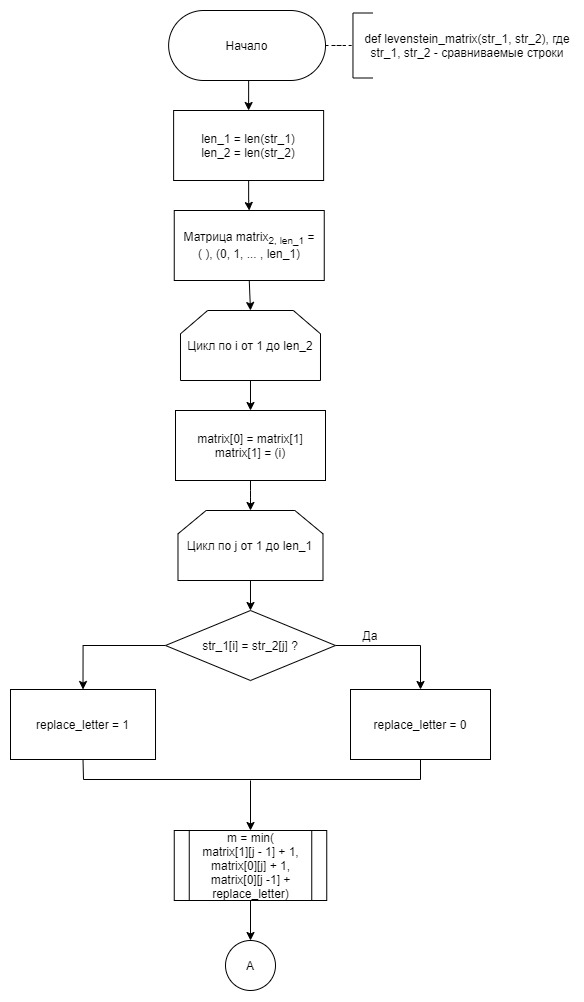
\includegraphics[scale=0.65]{inc/img/matrix_1.jpg}}
	\caption{Схема алгоритма нахождения расстояния Левенштейна - матричным способом (часть 1)}
	\label{img_matrix_1}
\end{figure}

\begin{figure}[h]
	\center{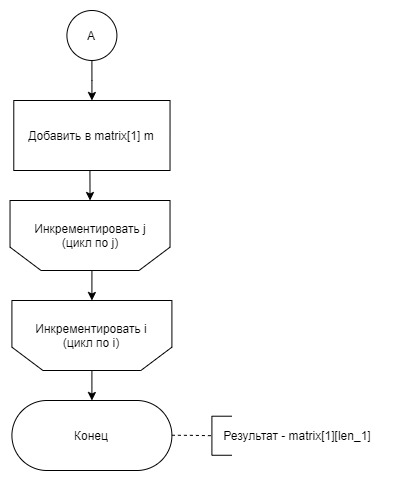
\includegraphics[scale=0.7]{inc/img/matrix_2.jpg}}
	\caption{Схема алгоритма нахождения расстояния Левенштейна - матричным способом (часть 2)}
	\label{img_matrix_2}
\end{figure}
\newpage

\section{Алгоритм нахождения расстояния Левенштейна - рекурсивно}
На рисунках \ref{img_rec_1} - \ref{img_rec_2} представлена схема алгоритма нахождения расстояния Левенштейна рекурсивно.
\begin{figure}[p]
	\center{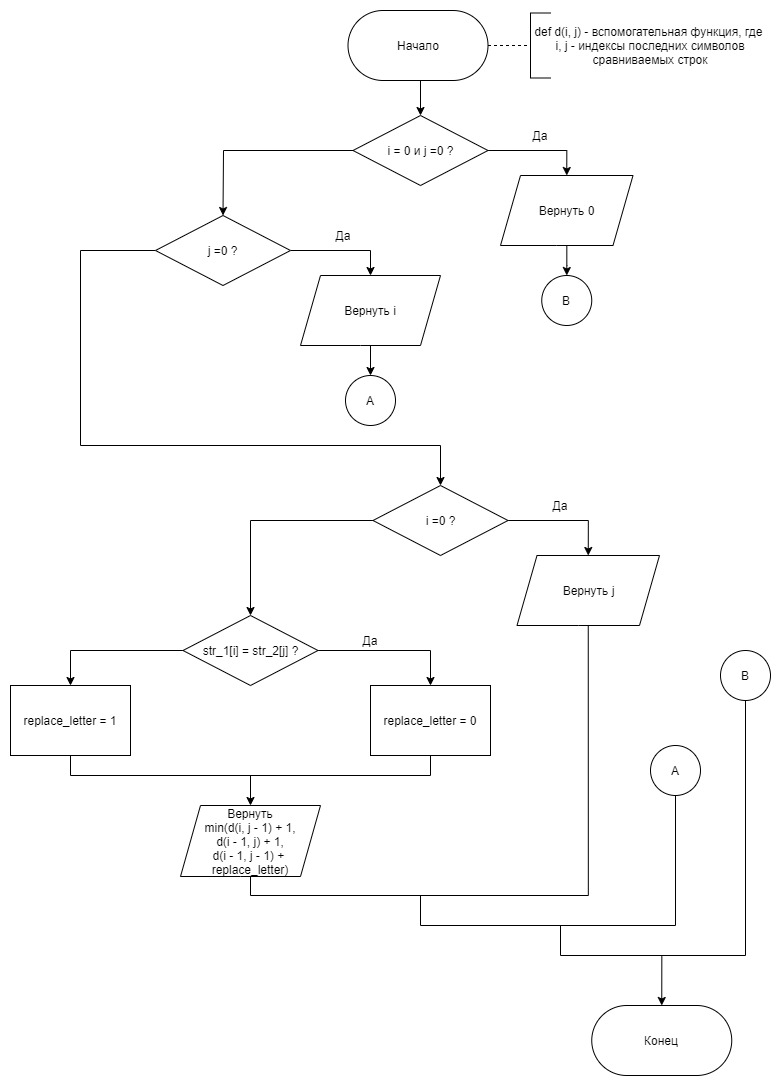
\includegraphics[scale=0.6]{inc/img/rec_1.jpg}}
	\caption{Схема алгоритма нахождения расстояния Левенштейна рекурсивно (часть 1)}
	\label{img_rec_1}
\end{figure}

\begin{figure}[h]
	\center{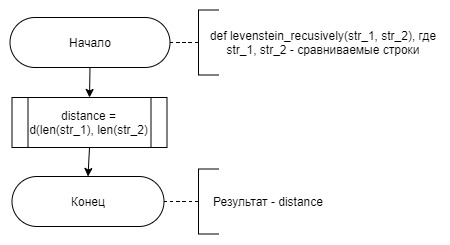
\includegraphics[scale=0.6]{inc/img/rec_2.jpg}}
	\caption{Схема алгоритма нахождения расстояния Левенштейна рекурсивно (часть 2)}
	\label{img_rec_2}
\end{figure}
\newpage

\section{Алгоритм нахождения расстояния Левенштейна - рекурсивно с использованием кэша}
На рисунках \ref{img_rec_cache_1} - \ref{img_rec_cache_3} представлена схема алгоритма нахождения расстояния Левенштейна рекурсивно с использованием кэширования.

\begin{figure}[p]
	\center{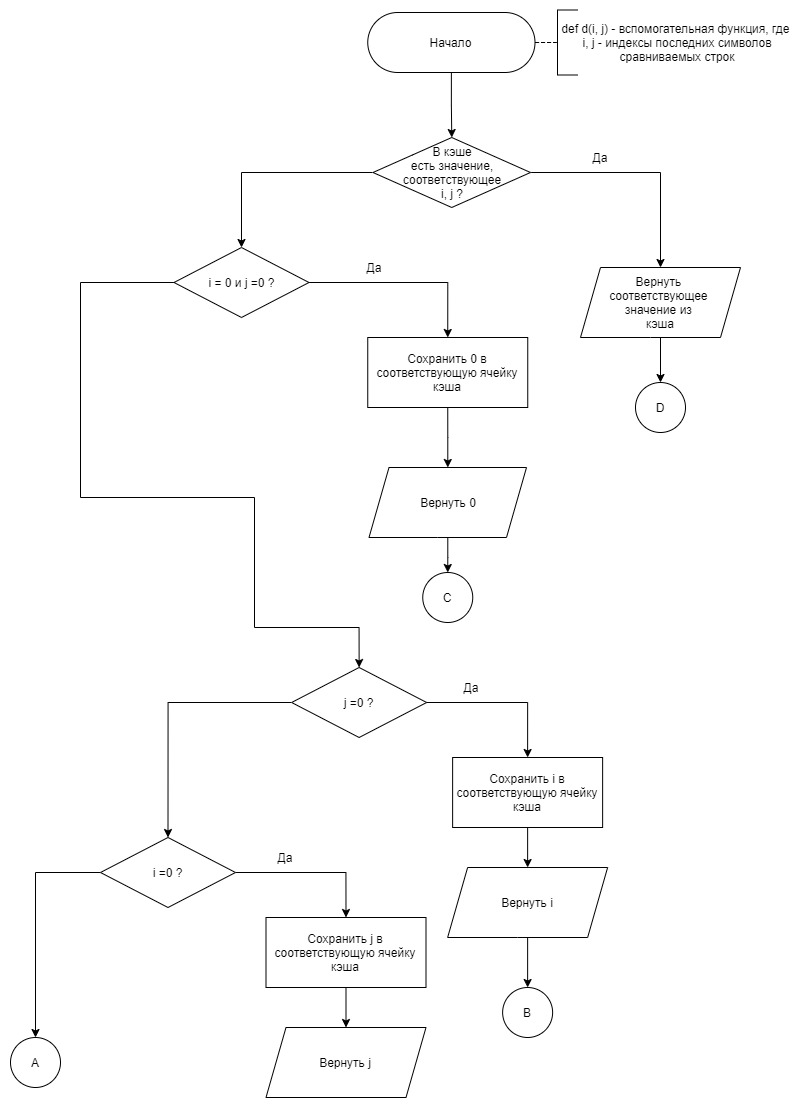
\includegraphics[scale=0.6]{inc/img/rec_cache_1.jpg}}
	\caption{Схема алгоритма нахождения расстояния Левенштейна рекурсивно с использованием кэша (часть 1)}
	\label{img_rec_cache_1}
\end{figure}
\begin{figure}[p]
	\center{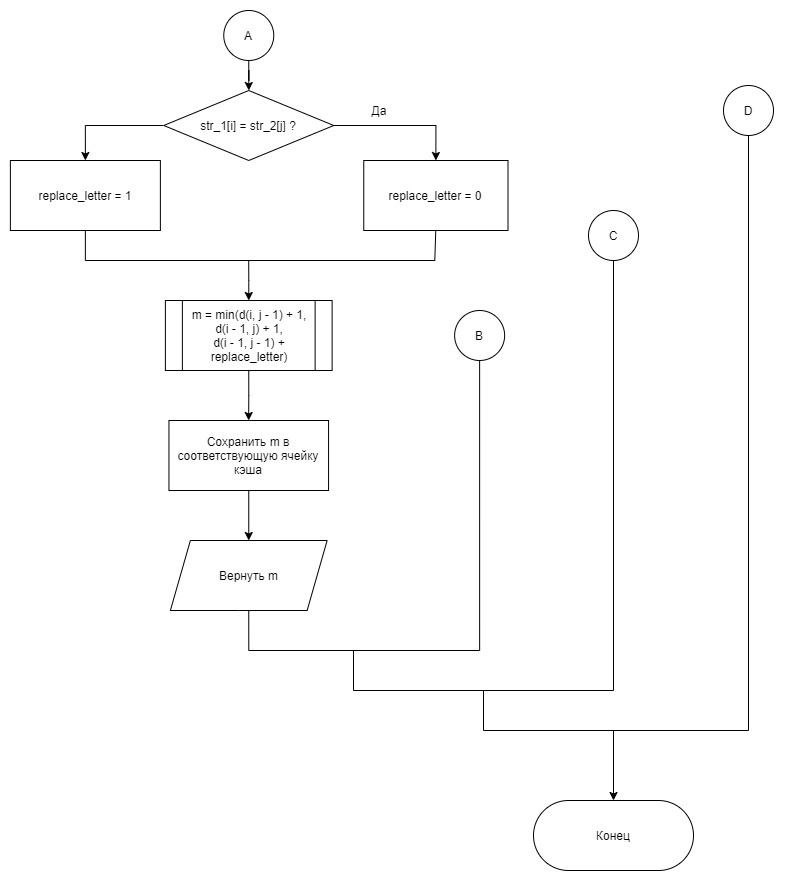
\includegraphics[scale=0.65]{inc/img/rec_cache_2.jpg}}
	\caption{Схема алгоритма нахождения расстояния Левенштейна рекурсивно с использованием кэша (часть 2)}
	\label{img_rec_cache_2}
\end{figure}
\begin{figure}[h]
	\center{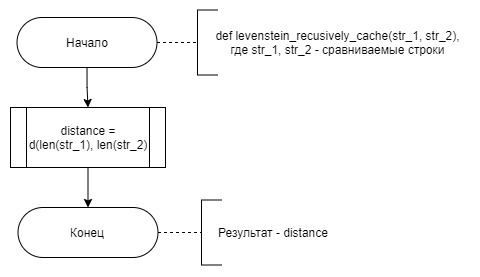
\includegraphics[scale=0.8]{inc/img/rec_cache_3.jpg}}
	\caption{Схема алгоритма нахождения расстояния Левенштейна рекурсивно с использованием кэша (часть 3)}
	\label{img_rec_cache_3}
\end{figure}
\newpage

\section{Алгоритм нахождения расстояния Дамерау-Левенштейна - рекурсивно}
На рисунках \ref{img_dam_1} - \ref{img_dam_3} представлена схема алгоритма нахождения расстояния Дамерау-Левенштейна рекурсивно.

\begin{figure}[p]
	\center{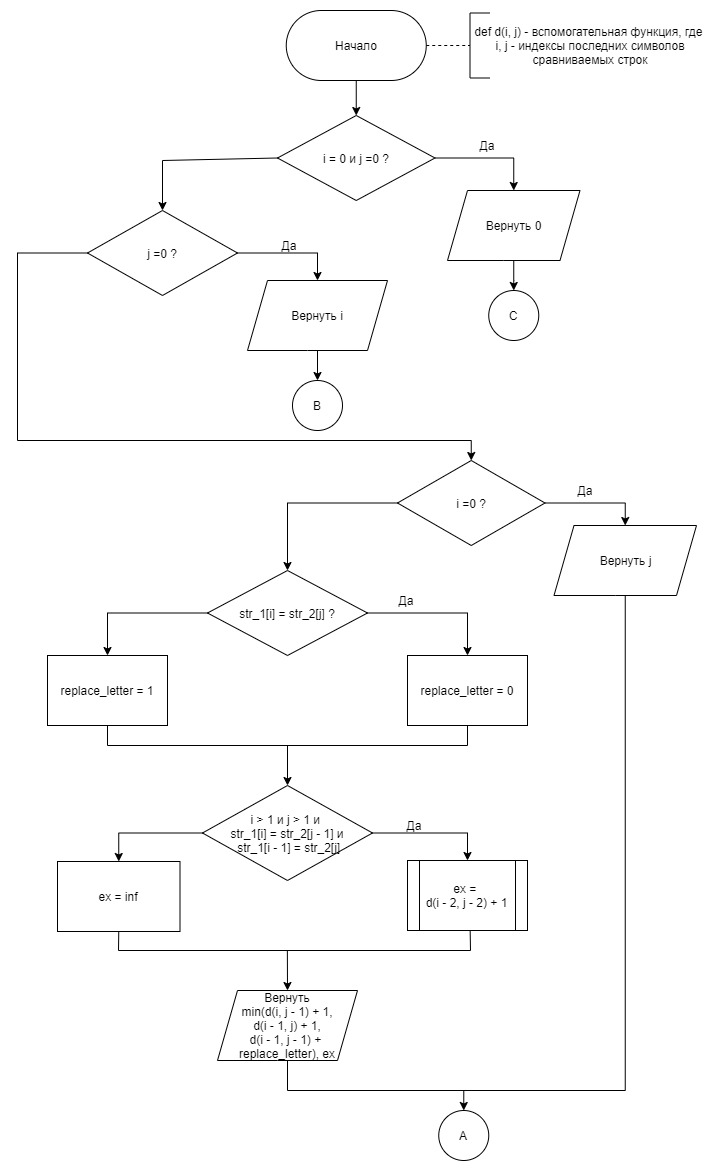
\includegraphics[scale=0.58]{inc/img/damerau_1.jpg}}
	\caption{Схема алгоритма нахождения расстояния Дамерау-Левенштейна рекурсивно (часть 1)}
	\label{img_dam_1}
\end{figure}
\begin{figure}[p]
	\center{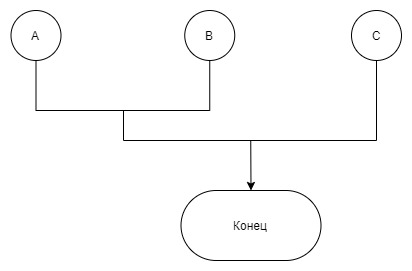
\includegraphics[scale=0.8]{inc/img/damerau_2.jpg}}
	\caption{Схема алгоритма нахождения расстояния Дамерау-Левенштейна рекурсивно (часть 2)}
	\label{img_dam_2}
\end{figure}
\begin{figure}[p]
	\center{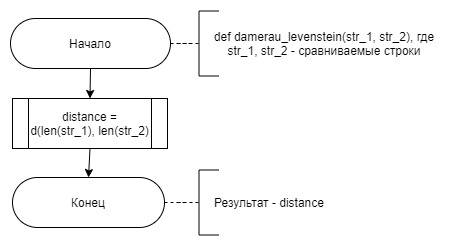
\includegraphics[scale=0.8]{inc/img/damerau_3.jpg}}
	\caption{Схема алгоритма нахождения расстояния Дамерау-Левенштейна рекурсивно (часть 3)}
	\label{img_dam_3}
\end{figure}
\newpage

\section{Вывод}
Таким образом, были разработаны схемы алгоритмов нахождения расстояния Левенштейна треми разными способами и расстояния Дамерау-Левенштейна - рекурсивно.
